\subsection{Memory}
\begin{frame}[fragile]
  \frametitle{GPU hardware: memory}
\begin{itemize}
\item GPU uses its own memory - {\color{mycolordef}global memory}
\item One might have to copy data between CPU host and GPU device.
\item K80 has 12G, V100 - 16G
\item The bandwidth between global memory and GPU for K80 is $480GB/s$, for V100 - $900GB/s$
\item For comparison: the typical bandwidth between CPU and RAM is about $100GB/s$
\item GPU card is typically connected to CPU host with PCI interface with a bandwidth of about $12GB/s$, for PCIe gen3 - $32GB/s$
\item There are faster interconnects  available, for example, {\color{mycolordef}NVlink} - $300GB/s$, but so far they are too expensive and not
  yet widespread and transferring data between CPU and GPU is likely to be the biggest bottleneck for a while
\item Therefore to get better performance, one needs to minimize moving data between the host and device or interleave it with the computations to hide the latency

\end{itemize}
\end{frame}


\begin{frame}[fragile]
  \frametitle{GPU hardware: memory}
\begin{itemize}
\item Given the number of threads, global memory is slow and one needs to minimize its usage as well
\item One way to optimize usage of global memory is {\color{mycolordef}coalescing}: take into account that data is read from global memory in {\color{mycolordef} aligned cache lines} and in ideal close threads should read close data
\item Per block, there is faster {\color{mycolordef}shared memory}, limited to $48k$ for K80 and $96k$ for V100. It can be used to cache global memory values manually.
\item Local variables in a thread are kept in {\color{mycolordef}registers} which are faster than shared memory. 
  However, there is limited amount of registers available and some local variables might spill into {\color{mycolordef}local memory} which physically resides in the same place as global
  memory and therefore is as slow.
\item {\color{mycolordef}Constant memory} is optimized for read operations although physically it is still the same as global memory.
\item {\color{mycolordef}Texture and surface memory} are used mostly for graphics programming and we shall not discuss it here.
\end{itemize}
\end{frame}


\begin{frame}[fragile]
  \frametitle{GPU hardware: memory}
\begin{columns}
\begin{column}{0.5\textwidth}
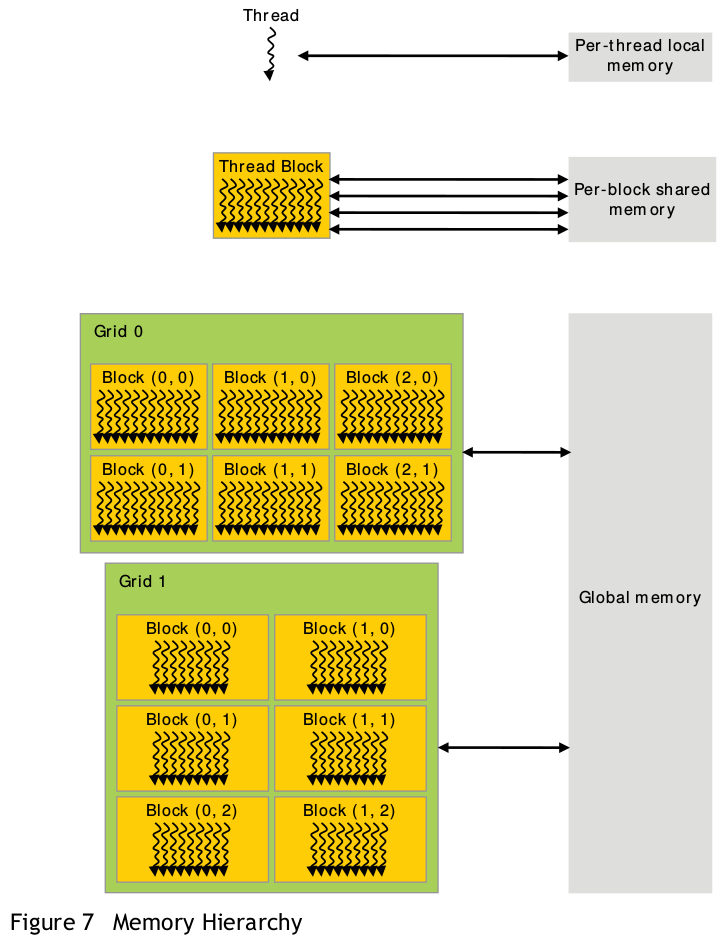
\includegraphics[width=6.0cm]{graphs/memory_hierarchy.png}
\end{column}
\begin{column}{0.5\textwidth}
\begin{itemize}
\item The host can only copy data to/from global, constant, texture, surface memory; not shared memory, registers or local memory
\item For optimal performance, it is important to {\color{mycolordef}align} data in memory since reads and writes start at aligned address
\item Builtin types are aligned automatically but user defined types like structures might have to be aligned manually
\end{itemize}
\end{column}
\end{columns}
\end{frame}

\begin{frame}[fragile]
  \frametitle{GPU hardware: memory}
\begin{columns}
\begin{column}{0.5\textwidth}
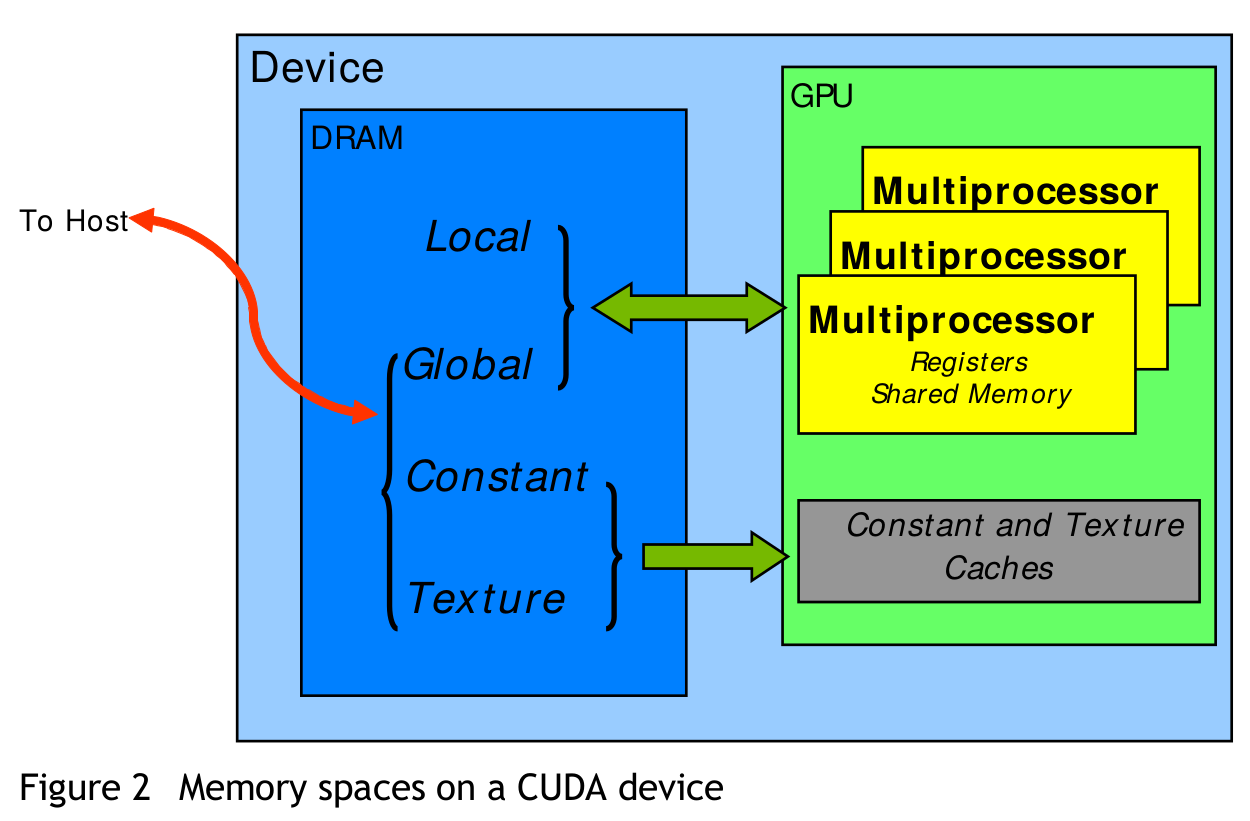
\includegraphics[width=4.0cm]{graphs/memory2.png}
\end{column}

\begin{column}{0.5\textwidth}
\begin{itemize}
\item {\color{mycolordef}Unified Memory}, available for $CC \ge 3.0$,  allows using the same pointer both on the host and device and makes data transfer transparent for the user. 
\end{itemize}
\end{column}

\end{columns}
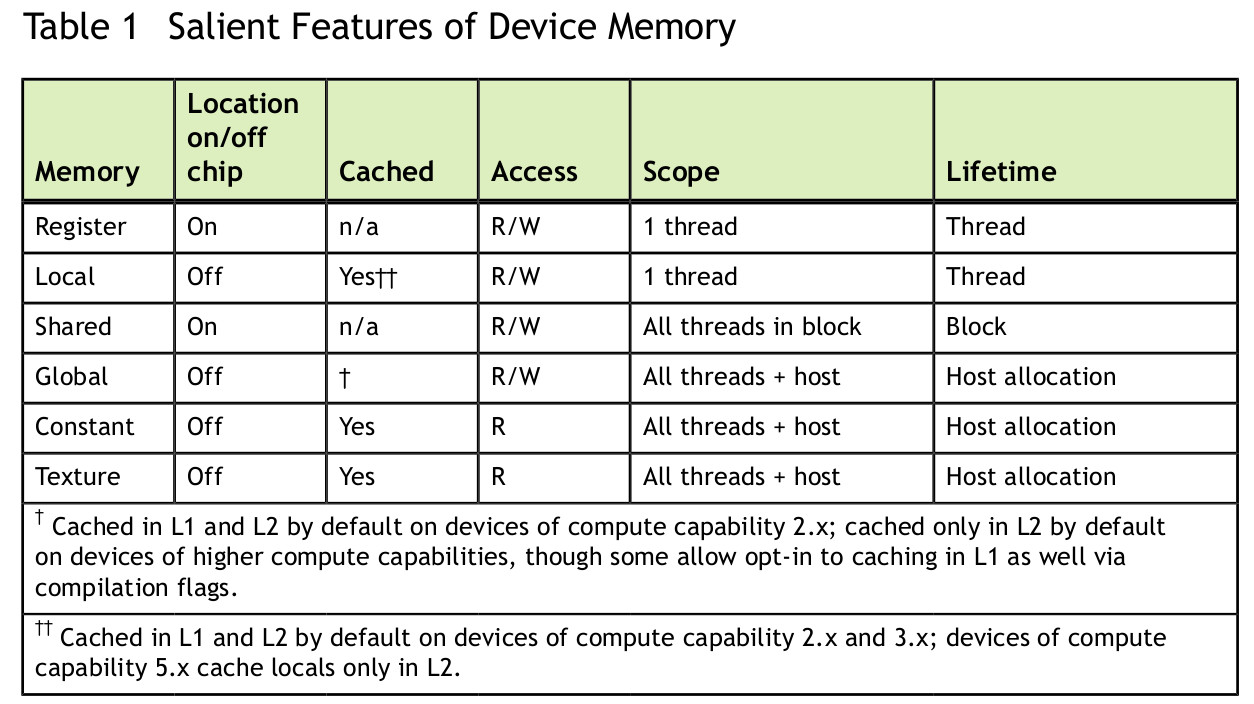
\includegraphics[width=9.0cm]{graphs/memory3.png}
\end{frame}


\begin{frame}[fragile]
  \frametitle{GPU hardware: memory}
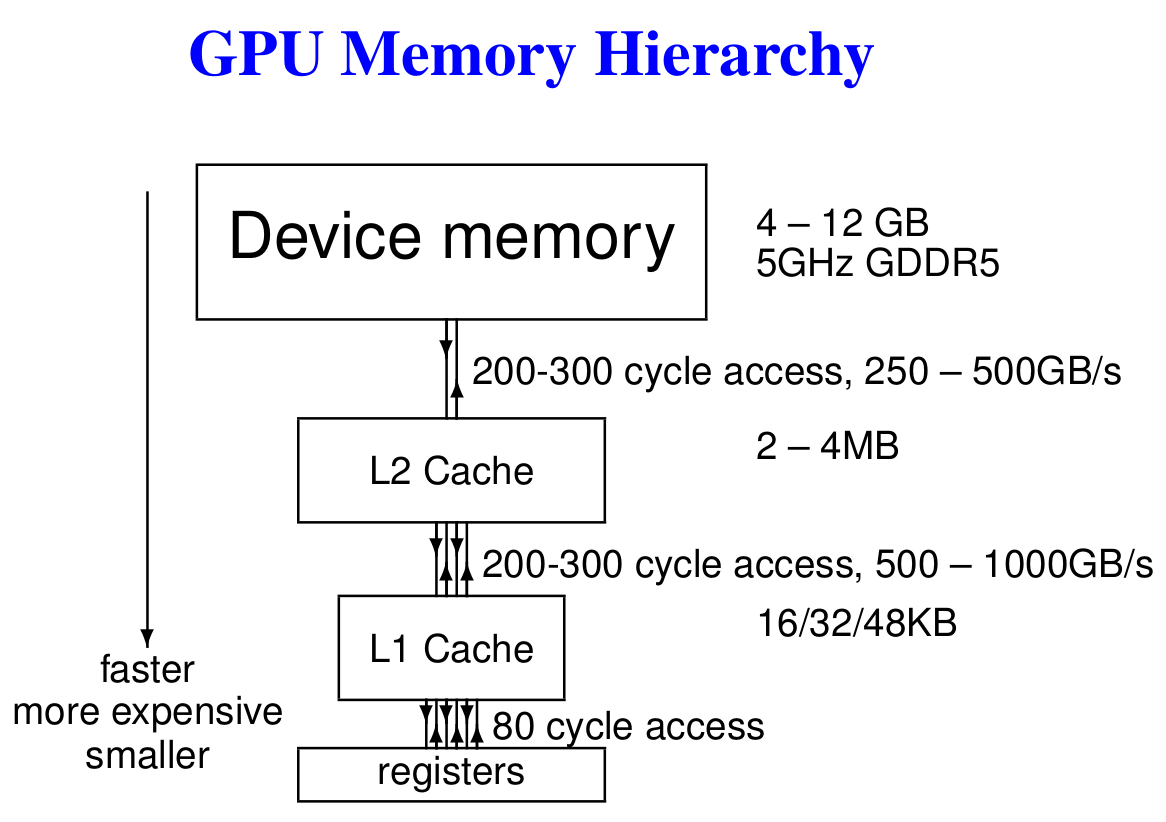
\includegraphics[width=11.0cm]{graphs/memory5.png}
\end{frame}

\begin{frame}[fragile]
  \frametitle{GPU hardware: memory}
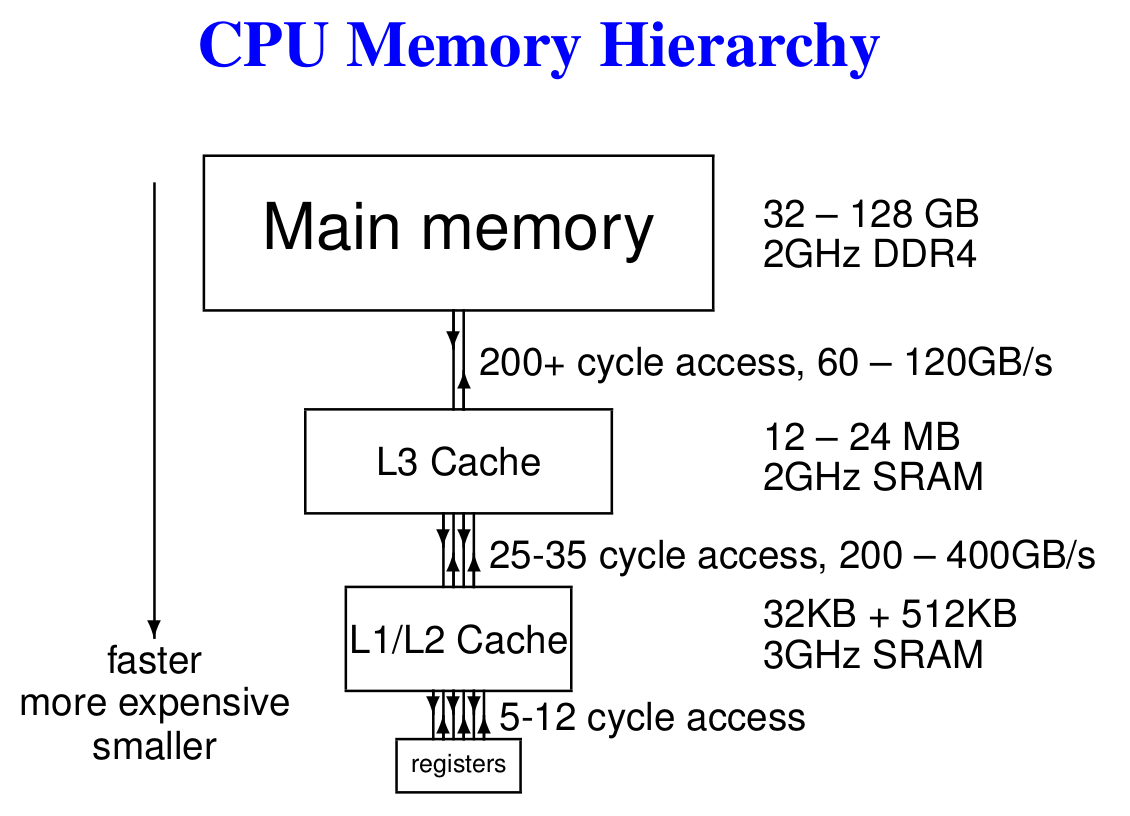
\includegraphics[width=11.0cm]{graphs/memory4.png}
\end{frame}